\chapter{多重积分}

多元函数积分学,根据多维空间为标量还是向量分为:
\begin{itemize}
    \item 多元数量值函数积分;
    \item 多元向量值函数积分。
\end{itemize}
本章简称“数量积分”和“向量积分”。
之前的一元函数积分学本章简称“一元积分”。

数量积分的物理应用对应诸如三维体质量、薄型平板电荷总量等。
数量积分是一元积分的多维扩展,被积函数从一元扩展到多元,微元也从一元扩展到多元。
通常来讲,被积函数是给出的,如三维体的体密度,不需要特别处理,关键要解决多维空间里微元的表达,解决了这个表达式,就能很容易化为一元积分。

本章介绍最基础的多重积分,多重积分是后续曲线积分和曲线积分的基础。

本章要点:
\begin{itemize}
    \item 多重积分的概念。
    \item 二重积分和三重积分的计算。
\end{itemize}

~

\newpage
\section{多元数量值函数积分的概念}

本节讨论多元数量积分的概念、性质、分类。

本节要点:
\begin{itemize}
    \item 掌握数量积分的概念;
    \item 掌握数量积分的性质。
\end{itemize}

%============================================================
\subsection{多元数量值函数积分的概念}

\begin{definition}[数量积分]
假设$\varOmega $为一可度量的有界的封闭几何体,函数$f$是定义在$\varOmega $上的一个有界的数量值函数,将$\varOmega $任意划分为$n$个小部分,并用$\Delta \varOmega _i$表示每一个小部分的度量,在每一个小部分上任取一点$M_i$,作乘积后再作和式:
\[
\sum_{i=1}^n{\left[ f\left( M_i \right) \cdot \Delta \varOmega _i \right]}
\]
记$\lambda =\max \left\{ diameter \ of \ \Delta \varOmega _i \right\} $,如果不论对$\varOmega $如何划分,也不论点$M_i$在$\varOmega $中如何选取,若当$\lambda \rightarrow 0$时上述和式有极限且相等,则称{\bf 函数$f$在$\varOmega $上可积},此极限值称为{\bf 多元数量值函数$f$在几何体$\varOmega $上的积分},记作$\int_{\varOmega}{f\left( M \right) d\varOmega}$,即:
\[
\int\limits_{\varOmega}{f\left( M \right) d\varOmega}:=\underset{\lambda \rightarrow 0}{\lim}\sum_{i=1}^n{\left[ f\left( M_i \right) \cdot \Delta \varOmega _i \right]}
\]
其中:
\begin{itemize}
    \item $\varOmega $:{\bf 积分区域},可以是二维、三维、甚至$n$维,并没有规定维度;
    \item $f$:{\bf 被积函数},是几何体$\varOmega $相应的维度的数量值函数,如果$\varOmega $是二维,则$f$是二元函数,如果$\varOmega $是三维,则$f$是三元函数。
\end{itemize}
\end{definition}

数学上,数量积分依旧是“加权和”的概念,$d\varOmega $对应加权$f\left( M \right) $后,在$\varOmega $范围内的和。

\begin{theorem}[存在性定理]
如果函数$f$在有界闭几何体$\varOmega $上是连续的,则$f$在$\varOmega $上必可积。
\end{theorem}

%============================================================
\subsection{多元数量值函数积分的性质和定理}

线性性:
\[
\int\limits_{\varOmega}{\left[ af\left( M \right) +bg\left( M \right) \right] d\varOmega}=a\int\limits_{\varOmega}{f\left( M \right) d\varOmega}+b\int\limits_{\varOmega}{g\left( M \right) d\varOmega}
\]

区域可加性:
\[
\int\limits_{\varOmega}{f\left( M \right) d\varOmega}=\int\limits_{\varOmega _1}{f\left( M \right) d\varOmega}+\int\limits_{\varOmega _2}{f\left( M \right) d\varOmega}
\]

不等式性质:
\[
f\left( M \right) \leqslant g\left( M \right) \quad \Rightarrow \quad \int\limits_{\varOmega}{f\left( M \right) d\varOmega}\leqslant \int\limits_{\varOmega}{g\left( M \right) d\varOmega}
\]

~

\begin{theorem}[估值定理]
设$m,M$分别是$f$在闭几何体$\varOmega $上的最小值和最大值,则:
\[
m\int\limits_{\varOmega}{d\varOmega}\leqslant \int\limits_{\varOmega}{f\left( M \right) d\varOmega}\leqslant M\int\limits_{\varOmega}{d\varOmega}
\]
\end{theorem}

\begin{theorem}[积分中值定理]
设$f$在闭几何体$\varOmega $上连续,则存在$M_0\in \varOmega $,有:
\[
\int\limits_{\varOmega}{f\left( M \right) d\varOmega}=f\left( M_0 \right) \int\limits_{\varOmega}{d\varOmega}
\]
\end{theorem}

\begin{theorem}[对称性定理]
当积分域$\varOmega $关于$x$对称时,
\begin{itemize}
    \item 若$f$关于$x=0$为奇函数,则$\int_{\varOmega}{f\left( M \right) d\varOmega}=0$;
    \item 若$f$关于$x=0$为偶函数,则$\int_{\varOmega}{f\left( M \right) d\varOmega}=2\int_{\varOmega '}{f\left( M \right) d\varOmega}$,其中$\varOmega '$为$\varOmega $ 位于$x<0$部分。
\end{itemize}
\end{theorem}






\newpage
\section{二重积分}

本节讨论二重积分的定义、意义和计算方法。

本节要点:
\begin{itemize}
    \item 掌握二重积分的定义;
    \item 了解二重积分的数学意义、物理意义和几何意义;
    \item 掌握二重积分在直角坐标下的计算方法;
    \item 了解二重积分在极坐标下的计算方法。
\end{itemize}

%============================================================
\subsection{二重积分的概念}

\begin{definition}[二重积分]
若$f\left( \boldsymbol{p} \right) $是定义在平面区域$D$上的二元数量值函数,则将{\bf $f\left( \boldsymbol{p} \right) $在$D$上的积分为二重积分}写成:
\begin{align*}
&\iint\limits_D{f\left( \boldsymbol{p} \right) d\sigma} \\
&D=\left\{ \left( x,y \right) \middle| x_1\leqslant x\leqslant x_2,y_1\left( x \right) \leqslant y\leqslant y_2\left( x \right) \right\}
\end{align*}
其中:
\begin{itemize}
    \item $f\left( \boldsymbol{p} \right) $:{\bf 被积函数};
    \item $d\sigma$:{\bf 积分微元};
    \item $D$:{\bf 积分区域}。
\end{itemize}
\end{definition}

这里需要注意一个地方。
$f\left( \boldsymbol{p} \right) $是一个二元数量值函数,也可以写成$z=z\left( x,y \right) $,$z$被$x,y$约束,$x,y$之间没有约束关系,反应几何上的一个曲面。
但是作为定积分,{\it xOy}平面上还是有一个积分区域的,它被一组曲线(或直线)包围,所以$y_1\left( x \right) \leqslant y\leqslant y_2\left( x \right) $描述的是这个积分区域,而不是$x,y$的约束关系。

%============================================================
\subsection{二重积分的几何意义和物理意义}

对比一元积分,二重积分在数学上是对一个指定平面的“加权和”。
\begin{align*}
&\int_a^b{f\left( x \right) dx} \quad x\in \left[ a,b \right] \\
&\iint\limits_D{f\left( \boldsymbol{p} \right) d\sigma} \quad D=\left\{ \left( x,y \right) \middle| x_1\leqslant x\leqslant x_2,y_1\left( x \right) \leqslant y\leqslant y_2\left( x \right) \right\}
\end{align*}
几何上,这个“权”可以由{\it z}轴表示,则二重积分的几何意义可以理解为以$D$为底、$f\left( \boldsymbol{p} \right) $为曲顶的曲顶柱体的体积。

物理上,如果这个“权”是密度,则二重积分表示这个指定平面的总质量,如果这个“权”是电荷密度,则二重积分表示这个指定平面的总电荷量。

\begin{figure}[h]
\centering
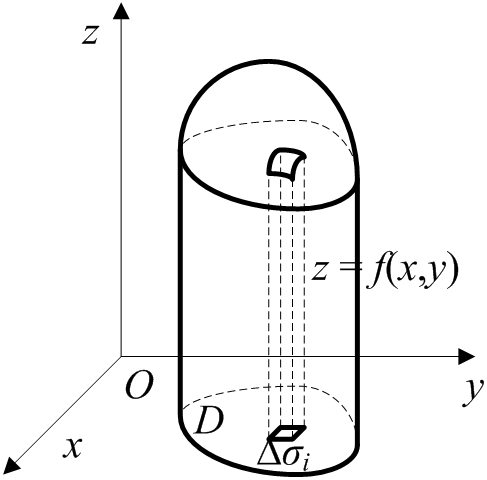
\includegraphics[height=4cm]{8.1.png}
\end{figure}

%============================================================
\subsection{二重积分的直角坐标计算}

总体来讲,二重积分的计算归根结底要化为一元积分,就是要将微元和被积函数都一元化。
在直角坐标下,面积微元可以表示为$d\sigma =dxdy$,于是:
\begin{align*}
&\iint\limits_D{f\left( \boldsymbol{p} \right) d\sigma}=\iint\limits_D{f\left( x,y \right) dxdy} \\
&D=\left\{ \left( x,y \right) \middle| x_1\leqslant x\leqslant x_2,y_1\left( x \right) \leqslant y\leqslant y_2\left( x \right) \right\}
\end{align*}
$D$可以理解为由两条直线$x=x_1,x=x_2$和两条曲线$y=y_1\left( x \right) ,y=y_2\left( x \right) $围成。
其次,将被积函数一元化。
曲顶柱体的体积的求解可以通过“切片”处理,先处理“一片”,再将“片”累加起来。

计算步骤:
\begin{enumerate}
    \item 计算$x_0$时的薄片的面积,即将$x_0$看成常数,求$y$从$y_1\left( x_0 \right) $到$y_2\left( x_0 \right) $的定积分,此时$f\left( x,y \right) $变为一元函数,薄片面积$S\left( x \right) $是$x$的函数
    \[
    S\left( x_0 \right) =\int_{y_1\left( x_0 \right)}^{y_2\left( x_0 \right)}{f\left( x_0,y \right) dy}
    \]
    \item 将这些薄片累积,即为该二重积分的结果
    \[
    \iint\limits_D{f\left( x,y \right) dxdy}=\int_{x_1}^{x_2}{S\left( x \right) dx}=\int_{x_1}^{x_2}{\left[ \int_{y_1\left( x \right)}^{y_2\left( x \right)}{f\left( x,y \right) dy} \right] dx}
    \]
\end{enumerate}

上式即为在直角坐标下二重积分$\iint_D{f\left( x,y \right)}$在区域$D$上的计算公式,常写作:
\begin{align*}
&\iint\limits_D{f\left( x,y \right) d\sigma}=\int_{x_1}^{x_2}{dx\int_{y_1\left( x \right)}^{y_2\left( x \right)}{f\left( x,y \right) dy}} \\
&D=\left\{ \left( x,y \right) \middle| x_1\leqslant x\leqslant x_2,y_1\left( x \right) \leqslant y\leqslant y_2\left( x \right) \right\}
\end{align*}
类似地,若积分区域$D$由两条直线$y=y_1,y=y_2$和两条曲线$x=x_1\left( y \right) ,x=x_2\left( y \right) $围成,则有:
\begin{align*}
&\iint\limits_D{f\left( x,y \right) d\sigma}=\int_{y_1}^{y_2}{dy\int_{x_1\left( y \right)}^{x_2\left( y \right)}{f\left( x,y \right) dx}} \\
&D=\left\{ \left( x,y \right) \middle| x_1\left( y \right) \leqslant x\leqslant x_2\left( y \right) ,y_1\leqslant y\leqslant y_2 \right\}
\end{align*}
最后要注意,如果积分区域$D$为凸区域,则二重积分结果和积分次序无关。

~

\begin{example}
计算$\iint_D{xyd\sigma}$,其中$D$由$y=x$和$y=x^2$围成。
\end{example}

解:

易得,围成的区域可以表示为$D=\left\{ \left( x,y \right) \middle| 0\leqslant x\leqslant 1,x^2\leqslant y\leqslant x \right\} $。
\begin{figure}[h]
\centering
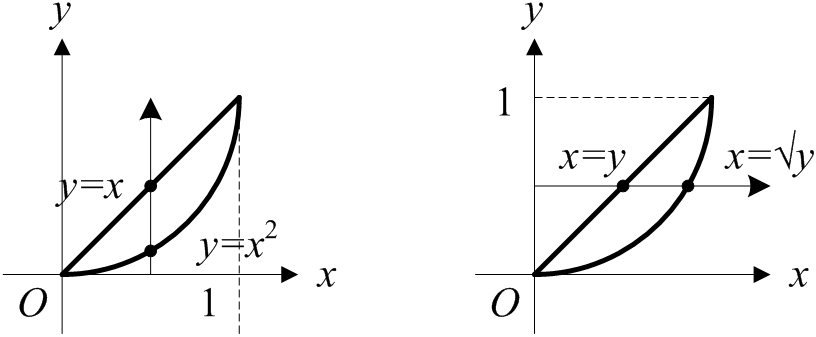
\includegraphics[height=3cm]{8.2.png}
\end{figure}
\begin{align*}
\iint\limits_D{f\left( x,y \right) d\sigma}&=\int_0^1{dx\int_{x^2}^x{xydy}}=\int_0^1{dx\left[ \left. \frac{1}{2}xy^2 \right|_{x^2}^{x} \right]} \\
&=\int_0^1{\left( \frac{1}{2}x^3-\frac{1}{2}x^5 \right) dx}=\frac{1}{24}
\end{align*}
也可以看成$D=\left\{ \left( x,y \right) \middle| y\leqslant x\leqslant \sqrt{y},0\leqslant y\leqslant 1 \right\} $:
\begin{align*}
\iint\limits_D{f\left( x,y \right) d\sigma}&=\int_0^1{dy\int_y^{\sqrt{y}}{xydx}}=\int_0^1{dy\left[ \left. \frac{1}{2}x^2y \right|_{y}^{\sqrt{y}} \right]} =\frac{1}{24}
\end{align*}

~

\begin{example}
求由柱面$x^2+y^2=R^2$和$x^2+z^2=R^2$所围成的立体(称为牟合立方)的体积。
\begin{figure}[ht]
\centering
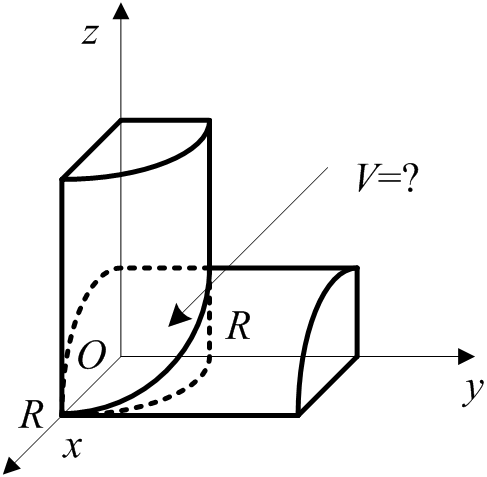
\includegraphics[height=3.5cm]{8.3.png}
\end{figure}
\end{example}

解:

以计算第一卦限为例。
该题可以理解成求一个均匀体的体积,可以用二重积分计算。
横的柱面的{\it z}轴值可以理解为高,纵的柱面在{\it xOy}平面的区域可以理解为积分区域,得到被积函数和积分区域:
\begin{align*}
&z\left( x,y \right) =\sqrt{R^2-x^2} \\
&D=\left\{ \left( x,y \right) \middle| 1\leqslant x\leqslant R,0\leqslant y\leqslant \sqrt{R^2-x^2} \right\}
\end{align*}
得到第一卦限部分的体积:
\begin{align*}
V&=\iint\limits_D{z\left( x,y \right) d\sigma}=\iint\limits_D{\sqrt{R^2-x^2}d\sigma} \\
&=\int_0^R{dx\int_0^{\sqrt{R^2-x^2}}{\sqrt{R^2-x^2}dy}}=\int_0^R{\left( R^2-x^2 \right) dx}=\frac{2}{3}R^2
\end{align*}

%============================================================
\subsection{二重积分的极坐标计算}

极坐标$\left( r,\theta \right) $的计算,在数学上和直角坐标一样:
\begin{align*}
&\iint\limits_D{f\left( r,\theta \right) d\sigma} \\
&D=\left\{ \left( r,\theta \right) \middle| \theta _1\leqslant \theta \leqslant \theta _2,r_1\left( \theta \right) \leqslant r\leqslant r_2\left( \theta \right) \right\}
\end{align*}
求解过程和直角坐标一样。
但如果方程以直角坐标的形式的给出,需要转换到极坐标。
这里,需要对变量进行变换以得到新的被积函数,还需要对$d\sigma $进行计算得到极坐标下的表达式。

坐标变换:
\[
\begin{cases}
	x=r\cos \theta\\
	y=r\sin \theta\\
\end{cases}
\]
微元$d\sigma $计算:
\begin{align*}
&\because \Delta \sigma =\frac{1}{2}\left( r+\Delta r \right) ^2\Delta \theta -\frac{1}{2}r^2\Delta \theta =r\Delta r\Delta \theta +\frac{1}{2}\Delta r^2\Delta \theta \\
&\therefore d\sigma =r\cdot drd\theta
\end{align*}
所以,直角坐标和极坐标的转换公式为:
\[
\iint\limits_D{f\left( x,y \right) dxdy}=\iint\limits_D{\left[ f\left( r\cos \theta ,r\sin \theta \right) \cdot r \right] drd\theta}
\]

二重积分,无论在直角坐标下计算,还是极坐标下计算,计算过程是一样的——“切片+累加”。
只是如果被积函数含有“弧状”(如$x^2+y^2$),极坐标下求解不定积分就会方便。

~

\begin{example}
计算以半径$R$的圆形为底,$H$为高的圆柱体体积。
\end{example}

解:

分析题干,相当于计算一个二重积分,被积函数恒为$H$,积分区域为一个圆,可假设该圆在圆心。
根据对称性,只要计算第一象限即可。
\[
V=4\iint\limits_D{Hd\sigma}=4\iint\limits_D{Hdxdy}
\]
直角坐标下,这个不定积分难解,换到极坐标就好解了。
将得到的式子转成极坐标求解:
\begin{align*}
V&=4\iint\limits_D{Hdxdy}=4\iint\limits_D{Hrdrd\theta}=4H\int_0^R{dr\int_0^{\pi /2}{rd\theta}} \\
&=4H\int_0^R{\frac{1}{2}\pi rdr}=\pi R^2H
\end{align*}
注意,这里虽然积分区域$D$没变,但是在极坐标下的表达式变了:
\begin{align*}
&D\left\{ \left( x,y \right) \middle| 0\leqslant x\leqslant R,0\leqslant y\leqslant \sqrt{R^2-x^2} \right\} \\
&\downarrow \\
&D\left\{ \left( r,\theta \right) \middle| 0\leqslant \theta \leqslant \frac{\pi}{2},0\leqslant r\leqslant R \right\}
\end{align*}






\newpage
\section{三重积分}

本节讨论三重积分的定义、意义和计算方法。

本节要点:
\begin{itemize}
    \item 掌握三重积分的定义;
    \item 了解三重积分的数学意义和物理意义;
    \item 掌握三重积分在直角坐标下的计算方法。
\end{itemize}

%============================================================
\subsection{三重积分的概念}

\begin{definition}[三重积分]
若$f\left( \boldsymbol{p} \right) $是定义在空间区域$V$上的三元数量值函数,则将{\bf $f\left( \boldsymbol{p} \right) $在$V$上的积分为三重积分}写成:
\begin{align*}
&\iiint\limits_V{f\left( \boldsymbol{p} \right) dv} \\
&V=\left\{ \left( x,y,z \right) \middle| x\in \left[ x_1,x_2 \right] ,y\in \left[ y_1\left( x \right) ,y_2\left( x \right) \right] ,z\in \left[ z_1\left( x,y \right) ,z_2\left( x,y \right) \right] \right\}
\end{align*}
其中:
\begin{itemize}
    \item $f\left( \boldsymbol{p} \right) $:{\bf 被积函数};
    \item $d\sigma$:{\bf 积分微元};
    \item $V$:{\bf 积分区域}。
\end{itemize}
\end{definition}

%============================================================
\subsection{三重积分的几何意义和物理意义}

对比一元积分和二重积分,三重积分在几何上是对一个指定三维空间的“加权和”。
\begin{align*}
&\int_a^b{f\left( x \right) dx} \quad x\in \left[ a,b \right] \\
&\iint\limits_D{f\left( \boldsymbol{p} \right) d\sigma} \quad D=\left\{ \left( x,y \right) \middle| x\in \left[ x_1,x_2 \right] ,y\in \left[ y_1,y_2 \right] \right\} \\
&\iiint\limits_V{f\left( \boldsymbol{p} \right) dv} \quad V=\left\{ \left( x,y,z \right) \middle| x\in \left[ x_1,x_2 \right] ,y\in \left[ y_1,y_2 \right] ,z\in \left[ z_1,z_2 \right] \right\}
\end{align*}

物理上,如果这个“权”是密度,则三重积分表示这个指定三维物体的总质量。
如果这个“权”是电荷密度,则三重积分表示这个指定三维物体的总电荷量。

%============================================================
\subsection{三重积分的直角坐标计算}

三重积分的计算思路和二重一样,将微元和被积函数都一元化。
被积函数一元化的方式依然采用“切片”方法。
在直角坐标下,体积微元可以表示为$dv=dxdydz$,于是:
\begin{align*}
&\iiint\limits_V{f\left( \boldsymbol{p} \right) dv}=\iiint\limits_V{f\left( x,y,z \right) dxdydz} \\
&V=\left\{ \left( x,y,z \right) \middle| x\in \left[ x_1,x_2 \right] ,y\in \left[ y_1\left( x \right) ,y_2\left( x \right) \right] ,z\in \left[ z_1\left( x,y \right) ,z_2\left( x,y \right) \right] \right\}
\end{align*}
三重积分的求解和二重积分类似,只是多了一个“切片”。

计算步骤:
\begin{enumerate}
    \item 先将$x_0,y_0$看成常数,对$z$求从$z_1\left( x_0,y_0 \right) $到$z_2\left( x_0,y_0 \right) $的定积分
    \[
    S\left( x_0,y_0 \right) =\int_{z_1\left( x_0,y_0 \right)}^{z_2\left( x_0,y_0 \right)}{f\left( x_0,y_0,z \right) dz}
    \]
    \item 再将该函数在$D$作二重积分
    \[
    \iint\limits_D{S\left( x,y \right) d\sigma}=\iint\limits_D{\left[ \int_{z_1\left( x,y \right)}^{z_2\left( x,y \right)}{f\left( x,y,z \right) dz} \right] d\sigma}
    \]
    或常写作:
    \[
    \iiint\limits_V{f\left( x,y,z \right) dv}=\iint\limits_D{dxdy\int_{z_1\left( x,y \right)}^{z_2\left( x,y \right)}{f\left( x,y,z \right) dz}}
    \]
\end{enumerate}

通过以上方法,化为了二重积分,后续过程略。
同样,三重积分可以在柱坐标和球坐标下计算。






\newpage
\section{多重积分的应用}

本节以物体中心为例说明多重积分的应用。

%============================================================
\subsection{物体重心}

重心即为对参考点的等效力矩的坐标。
取坐标原点为参考点。
假设三维体$\varOmega $有不均匀体密度$\rho \left( \boldsymbol{p} \right) $,则总重量:
\[
m=\iiint\limits_{\varOmega}{\rho \left( \boldsymbol{p} \right) d\sigma}
\]

首先考察三维体对{\it yOz}平面的总力矩:
\[
M_{yOz}=\iiint\limits_{\varOmega}{x\rho \left( \boldsymbol{p} \right) d\sigma}
\]
可得对于{\it yOz}平面的等效力矩的坐标:
\[
X=\frac{M_{yOz}}{m}=\frac{\iiint\limits_{\varOmega}{x\rho \left( \boldsymbol{p} \right) d\sigma}}{\iiint\limits_{\varOmega}{\rho \left( \boldsymbol{p} \right) d\sigma}}
\]

同理可得对于其他平面的等效力矩的坐标,略。






\newpage
\section{本章小结}

多重积分在数学上是一个$n$元函数在$n$维空间的积分。
\begin{figure}[h]
\centering
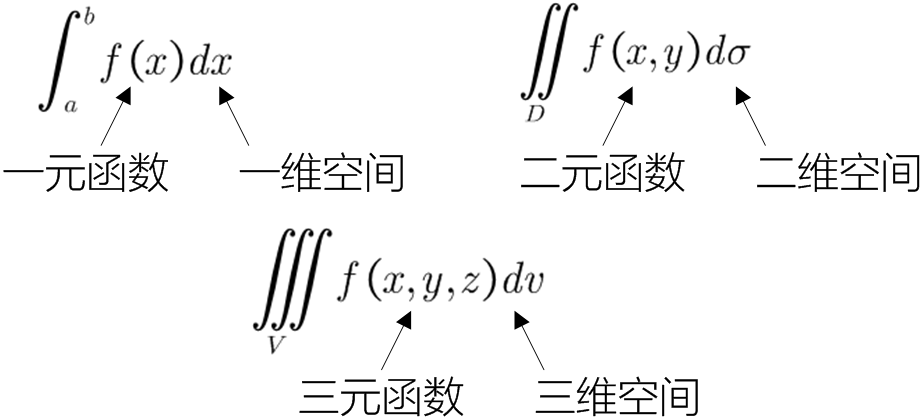
\includegraphics[height=3.5cm]{8.4.png}
\end{figure}

多重积分的物理意义非常简单明了,即已知$n$维体的体密度,求解该$n$维体的总重量。
如下表示线重量、面重量、体重量:
\begin{align*}
&W=\int_a^b{\rho \left( x \right) dx} \\
&W=\iint\limits_D{\rho \left( \boldsymbol{p} \right) d\sigma} \\
&W=\iiint\limits_V{\rho \left( \boldsymbol{p} \right) dv}
\end{align*}

多重积分的计算,总体步骤也非常明了:
\begin{enumerate}
    \item 固定$n-1$维,剩下一维变量进行积分,相当于求解一个一元函数积分,只是积分上下限是一个包含其余$n-1$维变量的表达式;
    \item 继续反复上面的步骤,直到剩下一维;
    \item 求解该一元积分。
\end{enumerate}
被积函数(即权重函数、或称密度函数)是给定的。
难点在于确定各个维度的积分上下限,即对于给定的积分区域求解各个维度的相互关系。









